\chapter{矩阵光学}

\section{傍轴状态空间与约定}

\section{光线状态}

取光轴为 \(z\) 轴，光线从左向右传播。在某一参考面上，以光线的高度 \(y\) 和与光轴的有向夹角 \(\alpha\) 作为状态变量：
\begin{equation}
	\vb r=
	\begin{pmatrix}
		y\\ \alpha
	\end{pmatrix},
	\qquad
	\alpha\simeq \frac{\dd y}{\dd z},
	\qquad
	|\alpha|\ll 1,\quad |y|/R\ll 1.
\end{equation}

这里的 \(\alpha\) 是几何角，而不是折射率乘以角度的约化角。若一个理想光具组把入射面 \(1\) 的状态变换到出射面 \(2\)，则在傍轴近似下有
\begin{equation}
	\vb r_2=M_{21}\vb r_1,\qquad
	M_{21}=
	\begin{pmatrix}
		A&B\\ C&D
	\end{pmatrix}.
\end{equation}
矩阵乘法按传播顺序从右向左进行：若先经过 \(M_1\)，再经过 \(M_2\)，总矩阵为 \(M_2M_1\).

本章主要采用几何角约定 \((y,\alpha)\). 在入射、出射介质折射率分别为 \(n_1,n_2\) 时，理想无损系统满足
\begin{equation}
	\det M_{21}=\frac{n_1}{n_2}.
\end{equation}
因此，在同一外部介质中 \(\det M=1\)，但在折射率改变的界面两侧不能不加说明地把 determinant 写成 \(1\).

另一个常用状态是约化角
\begin{equation}
	\vb s=
	\begin{pmatrix}
		y\\ u
	\end{pmatrix},
	\qquad u=n\alpha.
\end{equation}
令 \(P_n=\operatorname{diag}(1,n)\)，则
\begin{equation}
	\vb s_2=\widetilde M_{21}\vb s_1,\qquad
	\widetilde M_{21}=P_{n_2}M_{21}P_{n_1}^{-1},
\end{equation}
从而
\begin{equation}
	\det\widetilde M_{21}=1.
\end{equation}
	在这个约定中，两条近轴光线之间的光学不变量写成相空间面积形式
\begin{equation}
	\mathcal I
	=n\left(y_1\alpha_2-y_2\alpha_1\right)
	=y_1u_2-y_2u_1,
\end{equation}
	它在理想轴对称系统中保持不变；等价地说，系统矩阵在约化角状态中保持相空间面积。后文的主面、节点和 Gaussian beam 公式首先用几何角约定书写；若改用约化角，只需在系统的输入、输出端用上式作端点变换。

\section{传播、折射与反射的基本矩阵}

在折射率为 \(n\) 的均匀介质中传播距离 \(L\) 时，
\begin{equation}
	y'=y+L\alpha,\qquad \alpha'=\alpha,
\end{equation}
所以
\begin{equation}
	T_n(L)=
	\begin{pmatrix}
		1&L\\0&1
	\end{pmatrix},
\qquad
\widetilde T_n(L)=
	\begin{pmatrix}
		1&L/n\\0&1
	\end{pmatrix}.
\end{equation}
两种写法描述的是同一传播过程，只是第二种把角变量换成了 \(u=n\alpha\).

考虑曲率半径为 \(r\) 的球面界面，约定 \(r>0\) 表示球面凸向入射介质 \(n_1\) 一侧。设曲面处的法线相对于光轴的有向角为 \(\beta\)，则在顶点附近
\begin{equation}
	\beta\simeq-\frac{y}{r}.
\end{equation}
Snell 定律在一阶近似下为
\begin{equation}
	n_1(\alpha-\beta)=n_2(\alpha'-\beta).
\end{equation}
于是
\begin{equation}
	\alpha'=\frac{n_1-n_2}{n_2r}y+\frac{n_1}{n_2}\alpha,
\end{equation}
即
\begin{equation}
	R_{n_1\to n_2}(r)=
	\begin{pmatrix}
		1&0\\[2pt]
		\dfrac{n_1-n_2}{n_2r}&\dfrac{n_1}{n_2}
	\end{pmatrix},
\qquad
\det R_{n_1\to n_2}(r)=\frac{n_1}{n_2}.
\end{equation}
在约化角状态中，折射矩阵变成
\begin{equation}
	\widetilde R_{n_1\to n_2}(r)=
	\begin{pmatrix}
		1&0\\[2pt]
		\dfrac{n_1-n_2}{r}&1
	\end{pmatrix}.
\end{equation}
这个形式直接显示了折射对 \(y\) 的线性“光学功率”作用，也显示了为什么约化角约定的 determinant 总是 \(1\).

对于球面镜，在展开光路约定下，曲率半径为 \(R\) 的反射元件矩阵为
\begin{equation}
	M_{\mathrm{mirror}}(R)=
	\begin{pmatrix}
		1&0\\[2pt]
		-\dfrac{2}{R}&1
	\end{pmatrix}.
\end{equation}
这里的 \(R\) 应带有与展开方向相容的有向符号；若改用实际反射坐标，传播方向反转会改变坐标约定，不能直接把该矩阵逐字套用。

\section{薄透镜矩阵的物理来源}

在折射率为 \(n\) 的外部介质中，薄透镜可看作两个球面折射界面的极限。若透镜折射率为 \(n_\ell\)，两界面半径按通常的光学符号约定为 \(R_1,R_2\)，则薄透镜公式给出
\begin{equation}
	\frac{1}{f}
	=\left(\frac{n_\ell}{n}-1\right)
	\left(\frac{1}{R_1}-\frac{1}{R_2}\right).
\end{equation}
在同一外部介质的几何角约定中，透镜使光线角度改变
\begin{equation}
	\alpha'=\alpha-\frac{y}{f},
\end{equation}
所以
\begin{equation}
	L(f)=
	\begin{pmatrix}
		1&0\\[2pt]-\dfrac{1}{f}&1
	\end{pmatrix}.
\end{equation}
若透镜两侧介质不同，物方、像方焦距分别为 \(f,f'\)，则从物方主面 \(H\) 到像方主面 \(H'\) 的一般矩阵写成
\begin{equation}
	M_{HH'}=
	\begin{pmatrix}
		1&0\\[2pt]
		-\dfrac{1}{f'}&\dfrac{f}{f'}
	\end{pmatrix},
\qquad
\det M_{HH'}=\frac{f}{f'}=\frac{n_1}{n_2}.
\end{equation}
在同一介质中 \(f=f'\)，它退化为 \(L(f)\). 后文若未特别说明，透镜和光具组均处于同一外部介质中。

\section{复合系统不变量、主面、节点与焦点}

\section{一般复合矩阵}

设一个由传播、折射、反射和薄透镜组成的系统为
\begin{equation}
	M=
	\begin{pmatrix}
		a&b\\c&d
	\end{pmatrix}.
\end{equation}
矩阵元的物理意义需要结合参考面理解：\(a\) 是初始角度为零时的横向放大因子，\(b\) 是初始高度为零时的高度响应，\(c\) 是系统光学功率，\(d\) 是初始高度为零时的角度响应。特别地，
\begin{equation}
	c=0
\end{equation}
表示系统无有限焦点，是无焦系统；若 \(c\neq0\)，则后焦距和前焦距可由 \(c\) 及 determinant 读出。

对同一介质中的无损系统，\(\det M=ad-bc=1\). 对跨介质系统，记
\begin{equation}
	\Delta=ad-bc=\frac{n_1}{n_2}.
\end{equation}

\section{主面与焦点}

在输入、输出参考面分别向系统内部作有向平移 \(h,h'\)，使变换矩阵化为类薄透镜形式：
\begin{equation}
	T(h')\,M\,T(h)
	=
	\begin{pmatrix}
		1&0\\[2pt]-\dfrac{1}{f'}&\dfrac{f}{f'}
	\end{pmatrix}.
\end{equation}
这里的 \(h,h'\) 是代数距离；若图中把主面画在参考面右侧，则它们为正，若画在左侧则为负。直接比较矩阵元得到
\begin{align}
	h'&=\frac{1-a}{c},&
h&=\frac{ad-bc-d}{c},\label{eq:matrix-principal-plane}\\
	f'&=-\frac{1}{c},&
	f&=-\frac{\Delta}{c}.\label{eq:matrix-focal-length}
\end{align}
因此 \(f/f'=\Delta\)，正是光学不变量在焦距定义中的表现。

为了看清公式的来源，把平移写开：
\begin{equation}
	T(h')MT(h)=
	\begin{pmatrix}
	a+ch'&ah+b+h'(ch+d)\\
	c&ch+d
	\end{pmatrix}.
\end{equation}
令右上角为零、左上角为一，就得到式 \eqref{eq:matrix-principal-plane}.

相应地，若选择节点面 \(N,N'\)，使变换矩阵的右上角为零并且角度响应为一，则
\begin{equation}
	T(p')\,M\,T(p)=
	\begin{pmatrix}
		\Delta&0\\ c&1
	\end{pmatrix},
\end{equation}
其中
\begin{equation}
	p'=\frac{\Delta-a}{c},\qquad
	p=\frac{1-d}{c}.
\end{equation}
在同一介质中 \(\Delta=1\)，节点矩阵退化为薄透镜形式
\[
	\begin{pmatrix}1&0\\c&1\end{pmatrix},
\]
因此从物方节点到像方节点的有向角相同。跨介质时横向坐标会按 \(\Delta=n_1/n_2\) 缩放，不能把“节点处角度不变”误写成“横向高度不变”。

\begin{figure}[htbp]
	\centering
	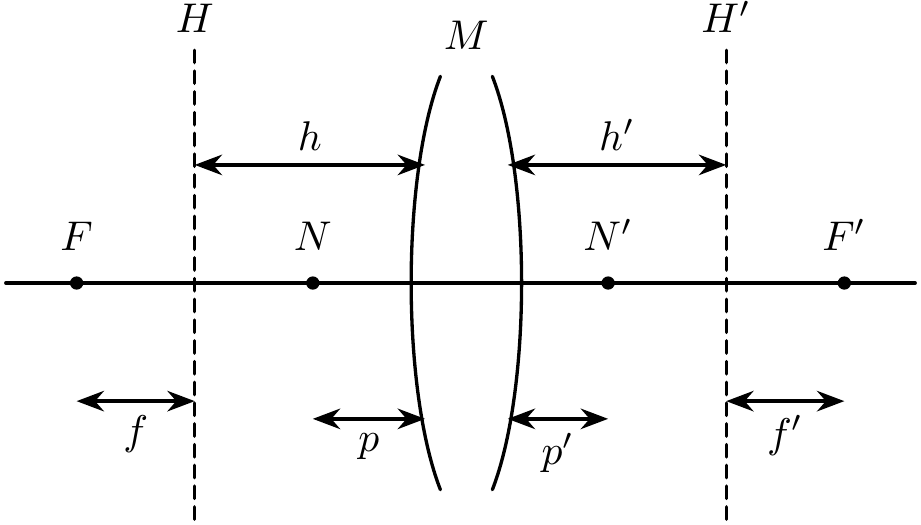
\includegraphics[width=0.72\textwidth]{matrix_optics_fig/principal_planes_nodes_and_foci.png}
	\caption{主面、节点和焦点的有向距离约定}
	\label{主面节点焦点图}
\end{figure}

\section{矩阵复合与验证例}

实际计算时只需按元件顺序相乘。以同一介质中的两个薄透镜为例，若透镜间距离为 \(d\)，则
\begin{equation}
	M_{2\mathrm{L}}=
	L(f_2)\,T(d)\,L(f_1)
	=
	\begin{pmatrix}
		1-\dfrac{d}{f_1}&d\\[6pt]
		-\dfrac{1}{f_1}-\dfrac{1}{f_2}+\dfrac{d}{f_1f_2}
		&1-\dfrac{d}{f_2}
	\end{pmatrix}.
\end{equation}
当 \(d=f_1+f_2\) 时，\(c=0\)，这就是 Kepler 型无焦光具组。其矩阵元直接给出横向和角度放大率，而不必先求所有主面。

下面保留三、四透镜的显式结果，作用是验证矩阵乘法、符号和 determinant；后文 Gaussian beam 与光腔计算只需要一般的 \(a,b,c,d\)，不再依赖这些长展开。

\begin{exbox}[title=三薄透镜验证例]
	设相邻透镜的净间距分别为 \(\Delta_1,\Delta_2\)，并记一般物方、像方介质中的第 \(i\) 个薄透镜矩阵为
	\[
		\mathcal L_i=
		\begin{pmatrix}
			1&0\\[2pt]-1/f_i'&f_i/f_i'
		\end{pmatrix}.
	\]
	则
	\begin{align*}
		M_{3\mathrm{L}}=
		\mathcal L_3\,T(\Delta_2+f_2'+f_3)\,
		\mathcal L_2\,T(\Delta_1+f_1'+f_2)\,\mathcal L_1.
	\end{align*}
	在一般物方、像方焦距记号下，其矩阵元为
	\begin{align*}
		a&=\frac{\Delta_1\Delta_2+\Delta_1f_3-f_2f_2'}{f_1'f_2'},\\
		b&=\frac{f_1}{f_1'f_2'}
		\Bigl(f_2f_2'-\Delta_1\Delta_2-\Delta_1f_3-f_1'\Delta_2-f_1'f_3\Bigr),\\
		c&=\frac{f_2f_2'-\Delta_1\Delta_2}{f_1'f_2'f_3'},\\
		d&=\frac{f_1}{f_1'f_2'f_3'}
		\Bigl(-f_2f_2'+\Delta_1\Delta_2+f_1'\Delta_2\Bigr),
		\qquad
		ad-bc=\frac{f_1f_2f_3}{f_1'f_2'f_3'}.
	\end{align*}
	在同一介质中令 \(f_i=f_i'\)，最后一式退化为 \(ad-bc=1\).
\end{exbox}

\begin{exbox}[title=四薄透镜验证例]
	同理，四透镜系统可写成
	\begin{align*}
		M_{4\mathrm{L}}
		={}\mathcal L_4\,T(\Delta_3+f_3'+f_4)\,
		\mathcal L_3\,T(\Delta_2+f_2'+f_3)\\
		&\times\mathcal L_2\,T(\Delta_1+f_1'+f_2)\,\mathcal L_1.
	\end{align*}
	其矩阵元为
	\begin{align*}
		a={}&\frac{1}{f_1'f_2'f_3'}
		\Bigl(\Delta_1f_3f_3'+(\Delta_3+f_4)(f_2f_2'-\Delta_1\Delta_2)\Bigr),\\
		b={}&\frac{f_1}{f_1'f_2'f_3'}
		\Bigl(-f_3f_3'(\Delta_1+f_1')
		+(\Delta_3+f_4)(-f_2f_2'+\Delta_1\Delta_2+f_1'\Delta_2)\Bigr),\\
		c={}&-\frac{1}{f_1'f_2'f_3'f_4'}
		\Bigl(\Delta_1f_3f_3'+\Delta_3f_2f_2'
		-\Delta_1\Delta_2\Delta_3\Bigr),\\
		d={}&\frac{f_1}{f_1'f_2'f_3'f_4'}
		\Bigl(f_3f_3'(\Delta_1+f_1')
		-\Delta_3(-f_2f_2'+\Delta_1\Delta_2+f_1'\Delta_2)\Bigr),\\
		&\hspace{2cm}
		ad-bc=\frac{f_1f_2f_3f_4}{f_1'f_2'f_3'f_4'}.
	\end{align*}
\end{exbox}

\section{Gaussian beam 的 \(q\) 参数与 ABCD 变换}

\section{从傍轴波动方程到复参数}

取时间因子为 \(e^{-\mathrm i\omega t}\)，写标量场为
\[
	\mathcal E(\vb r,t)=U(x,y,z)e^{\mathrm i k z-\mathrm i\omega t}.
\]
将 Helmholtz 方程在 \(U\) 缓慢变化的条件下截断，得到傍轴波动方程
\begin{equation}
	\left(\nabla_\perp^2+2\mathrm i k\frac{\partial}{\partial z}\right)U=0,
\qquad
	\left|\frac{\partial^2U}{\partial z^2}\right|
	\ll
	k\left|\frac{\partial U}{\partial z}\right|.
\end{equation}
其最低阶圆对称解可写成
\begin{equation}
	U(r,z)=U_0\frac{w_0}{w(z)}
	\exp\!\left(\mathrm i k z-\frac{\mathrm i k r^2}{2q(z)}
	-\mathrm i\zeta(z)\right),
\end{equation}
其中
\begin{align}
	q(z)&=z+\mathrm i z_R,\qquad
	\frac{1}{q(z)}=\frac{1}{R(z)}
	-\frac{2\mathrm i}{k w(z)^2},\\
	w(z)^2&=w_0^2\left(1+\frac{z^2}{z_R^2}\right),&
	R(z)&=\frac{z^2+z_R^2}{z},&
\zeta(z)&=\arctan\frac{z}{z_R},\\
	z_R&=\frac{k w_0^2}{2}.
\end{align}
\(z_R\) 是 Rayleigh 距离，也就是束腰到 \(w=\sqrt2w_0\) 的距离。原文中使用的复曲率
\begin{equation}
	\rho(z)=z-\mathrm i z_R
\end{equation}
正是 \(q(z)^*\)，并满足
\begin{equation}
	\frac{1}{\rho}=\frac{1}{R}+\frac{2\mathrm i}{k w^2}.
\end{equation}
两种记号完全等价；下面优先使用标准的 \(q\) 记号，以便直接写出 ABCD 变换。

\begin{figure}[htbp]
	\centering
	
\includegraphics[width=0.78\textwidth]{matrix_optics_fig/gaussian_beam_through_lens_group.png}
	\caption{Gaussian beam 通过理想光具组}
	\label{高斯光束通过透镜组}
\end{figure}

\section{几何光线与 Gaussian beam 的联系}

在几何光学中，同一球面波面上光线满足
\begin{equation}
	\alpha\simeq \frac{y}{R}.
\end{equation}
	在纯几何极限中 \(\rho=R\)；有限束腰时，\(\rho\) 是几何曲率半径的复化，而 \(1/\rho\) 的实部描述波前曲率，虚部描述有限束腰引入的衍射发散。令
\[
	\rho=\frac{y}{\alpha}
\]
并对任意实矩阵 \(M=\begin{pmatrix}A&B\\C&D\end{pmatrix}\) 变换，就有
\begin{equation}
	\rho_2=\frac{A\rho_1+B}{C\rho_1+D}.
\end{equation}
由于 \(q=\rho^*\) 且 \(A,B,C,D\) 为实数，Gaussian beam 的复参数同样满足 Möbius 变换
\begin{equation}
	\boxed{\displaystyle
	q_2=\frac{Aq_1+B}{Cq_1+D}}.
\label{eq:q-abcd}
\end{equation}

式 \eqref{eq:q-abcd} 使用局部波数 \(k=nk_0\) 定义 \(q\). 因而平面折射界面的矩阵
\[
	\begin{pmatrix}1&0\\0&n_1/n_2\end{pmatrix}
\]
给出 \(q_2=(n_2/n_1)q_1\)，这正是 \(z_R\propto n\) 的变化。若使用约化角矩阵，必须同步变换输入、输出的 \(q\) 定义，不能把两种状态约定混写。

\section{实部、虚部和束腰位置}

设系统矩阵为
\begin{equation}
	M=
	\begin{pmatrix}A&B\\C&D\end{pmatrix},
\qquad \Delta=AD-BC,
\end{equation}
入射面上的复参数为
\[
	q_1=x_1+\mathrm i z_{R1}.
\]
由式 \eqref{eq:q-abcd} 直接得到
\begin{align}
	\Re q_2&=
	\frac{(Ax_1+B)(Cx_1+D)+ACz_{R1}^2}
	{(Cx_1+D)^2+C^2z_{R1}^2},\\
\Im q_2&=
	\frac{z_{R1}\Delta}
	{(Cx_1+D)^2+C^2z_{R1}^2}.
\end{align}
若输出参考面之后再自由传播距离 \(z_2\)，并记输出束腰相对于该参考面的坐标为 \(z_{02}\)，则
\begin{equation}
	q_2(z_2)=z_2-z_{02}+\mathrm i z_{R2}.
\end{equation}
于是，若入射束腰相对于输入参考面的坐标为 \(z_{01}\)，即 \(q_1=z_{01}+\mathrm i z_{R1}\)，则
\begin{align}
	z_{R2}
	&=\frac{z_{R1}\Delta}
	{z_{R1}^2C^2+(Cz_{01}+D)^2},\\
	z_{02}
	&=-\frac{z_{R1}^2AC+(Az_{01}+B)(Cz_{01}+D)}
	{z_{R1}^2C^2+(Cz_{01}+D)^2}.
\end{align}
若 \(C=0\)，系统无焦，束腰位置的表达式相应简化为线性传播和横向缩放。

用主面和焦距表示时，令
\[
	Z_1=z_{01}-h,\qquad Z_2=z_{02}-h',
\]
则
\begin{align}
	Z_2&=
	\frac{f'\bigl(z_{R1}^2-Z_1(f-Z_1)\bigr)}
	{z_{R1}^2+(f-Z_1)^2},\\
	z_{R2}&=
	\frac{z_{R1}ff'}
	{z_{R1}^2+(f-Z_1)^2}.
\end{align}
恢复参考面的坐标即
\begin{align}
	z_{02}&=h'
	+\frac{f'\bigl(z_{R1}^2-(z_{01}-h)(f-z_{01}+h)\bigr)}
	{z_{R1}^2+(f-z_{01}+h)^2},\\
	z_{R2}&=
	\frac{z_{R1}ff'}
	{z_{R1}^2+(f-z_{01}+h)^2}.
\end{align}
比较这些表达式在 \(z_{R1}\to0\) 时的极限，可得
\begin{equation}
	(Z_2-f')(Z_1-f)
	=
	ff'\,
	\frac{(Z_1-f)^2}{z_{R1}^2+(Z_1-f)^2}.
\end{equation}
因此 Gaussian beam 的束腰位置只满足修正的 Newton 关系；只有在几何光学极限 \(z_{R1}\to0\) 下才恢复
\[
	(Z_2-f')(Z_1-f)=ff'.
\]

\section{光腔稳定性}

把反射后的光路展开后，设一个往返传播的矩阵为
\begin{equation}
	M_{\mathrm{rt}}=
	\begin{pmatrix}
	A&B\\C&D
	\end{pmatrix},
\qquad
\det M_{\mathrm{rt}}=1.
\end{equation}
腔内稳定 Gaussian mode 必须在一次往返后回到同一个 \(q\)，所以
\begin{equation}
	q=\frac{Aq+B}{Cq+D},
\end{equation}
即
\begin{equation}
	Cq^2+(D-A)q-B=0.
\end{equation}
当 \(C\neq0\) 时，
\begin{equation}
	q=\frac{A-D\pm\sqrt{(A+D)^2-4}}{2C}.
\end{equation}
由于 \(\det M_{\mathrm{rt}}=1\)，存在具有 \(\Im q>0\) 的物理解当且仅当
\begin{equation}
	\left|\frac{A+D}{2}\right|<1.
\label{eq:cavity-stability}
\end{equation}
等号对应边界稳定，实际腔中会对孔径、镜面误差和衍射损耗极其敏感；不等式失效时，往返变换没有正常的有限束腰。

以长度为 \(L\)、两球面镜曲率半径为 \(R_1,R_2\) 的二镜腔为例，定义
\begin{equation}
	g_1=1-\frac{L}{R_1},\qquad
	g_2=1-\frac{L}{R_2}.
\end{equation}
使用自由传播矩阵和镜面矩阵
\[
	T(L)=\begin{pmatrix}1&L\\0&1\end{pmatrix},
\qquad
	M_{\mathrm{mirror}}(R_i)=
	\begin{pmatrix}1&0\\-2/R_i&1\end{pmatrix},
\]
可得往返矩阵的半迹为
\begin{equation}
	\frac{\operatorname{Tr}M_{\mathrm{rt}}}{2}=2g_1g_2-1.
\end{equation}
于是式 \eqref{eq:cavity-stability} 退化为熟知的稳定性条件
\begin{equation}
	0<g_1g_2<1.
\end{equation}
若腔在两个横向方向上不再轴对称，应对 \(x,y\) 两个方向分别建立矩阵。

\section{完整光具组实例：两透镜四焦面 relay}

考虑焦距分别为 \(f_1,f_2\) 的两个薄透镜，透镜间距取为
\[
	d=f_1+f_2.
\]
先在两透镜主面之间计算系统矩阵：
\begin{equation}
	M_{\mathrm{lens}}=
	L(f_2)T(f_1+f_2)L(f_1)
	=
	\begin{pmatrix}
		-\dfrac{f_2}{f_1}&f_1+f_2\\[6pt]
		0&-\dfrac{f_1}{f_2}
	\end{pmatrix}.
\end{equation}
因为 \(c=0\)，系统是无焦的；它把平行入射光变成平行出射光，同时完成横向和角度的反向缩放。

若把输入面取在第一片透镜的前焦面，把输出面取在第二片透镜的后焦面，则总矩阵为
\begin{align}
	M_{\mathrm{4f}}
	&=T(f_2)L(f_2)T(f_1+f_2)L(f_1)T(f_1)\\
	&=
	\begin{pmatrix}
		-\dfrac{f_2}{f_1}&0\\[6pt]
		0&-\dfrac{f_1}{f_2}
	\end{pmatrix}.
\end{align}
因此
\begin{equation}
	y_{\mathrm{out}}=-\frac{f_2}{f_1}y_{\mathrm{in}},
\qquad
\alpha_{\mathrm{out}}=-\frac{f_1}{f_2}\alpha_{\mathrm{in}},
\qquad
\det M_{\mathrm{4f}}=1.
\end{equation}
横向放大率和角放大率互为倒数，正是光学不变量的直接体现。两透镜之间的中间平面是 Fourier 平面：矩阵光学给出其傍轴几何映射，而该平面上的空间频率分布和孔径滤波需要由 Fourier 光学继续处理。

对 Gaussian beam，式 \eqref{eq:q-abcd} 给出
\begin{equation}
	q_{\mathrm{out}}
	=\frac{f_2^2}{f_1^2}\,q_{\mathrm{in}}.
\end{equation}
所以
\begin{equation}
	z_{R,\mathrm{out}}=\frac{f_2^2}{f_1^2}z_{R,\mathrm{in}},
\qquad
	w_{0,\mathrm{out}}=\left|\frac{f_2}{f_1}\right|w_{0,\mathrm{in}},
\end{equation}
在同一波长、同一外部介质中成立。若 \(f_1=50\,\mathrm{mm}\)、\(f_2=200\,\mathrm{mm}\)，则横向放大率为 \(-4\)，角放大率为 \(-1/4\)，Rayleigh 距离放大为 \(16\)，束腰半径放大为 \(4\).
